% Chapter Template

\chapter{Chapter title} % Main chapter title
\label{Chapter1} % Change X to a consecutive number; for referencing this chapter elsewhere, use \ref{ChapterX}
%\lhead{Chapter One. \emph{Background and Introduction}} % Change X to a consecutive number; this is for the header on each page - perhaps a shortened title

%---------------------------------------------------------------------------------------
%	SECTION 1
%---------------------------------------------------------------------------------------
\section{Section title} % or comment this out and input from files (next line)
%\input{./Chapters/Chap1_Section1}

background information and literature review \cite{ffowcs:63}

figure example Fig.~\ref{f:example}
\begin{figure}[h!]
    \centering
    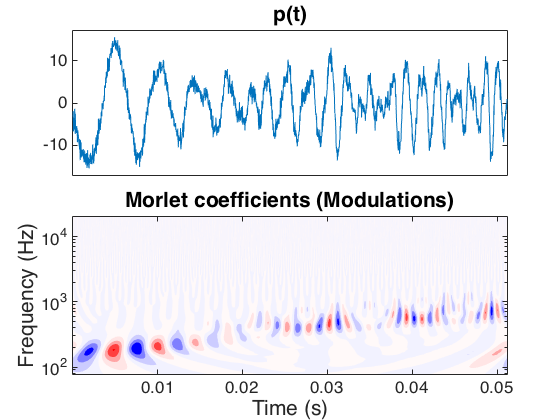
\includegraphics[width=.5\textwidth]{Morlet_real.png}
    \caption{Here goes the caption}
    \label{f:example}
\end{figure}
